\chapter{Procesamiento señal de voz}
En este capítulo conoceremos más acerca del procedimiento para procesar la señal de voz, además repasaremos algunos conceptos previos para entender en procesamiento y luego introduciremos 2 conceptos importantes \textit{Extracción de características y la coincidencia de patrones.}

\section{Conceptos previos}
\subsection{Voz}
Los seres humanos diariamente nos comunicamos por medio del habla utilizando nuestras voces somos capaces de transferir información en forma de \textit{ondas sonoras}.\\ Estas ondas transmiten una gran cantidad de información usando el aire como medio de transmisión.
Las propiedades como variaciones en amplitud al empezar o finalizar una palabra varían en el transcurso del tiempo, por lo cual es importante analizar segmentos de tiempo donde estas propiedades se mantengan aisladas de esta manera nos aseguramos que la señal de voz no cambie.
\subsection{Audios}
Los audios son un tipo de \textit{datos no estructurados}, es decir datos que no se encuentran en algún tipo de estructura de datos, estos tipos de datos son los que más se encuentran el mundo real como imágenes y audio. Una características de estos es que son complejos en su recolección y preparación para la realización de un análisis.\\ El audio puede capturarse mediante la grabación de nuestro entorno pero para que este audio sea entendido por las computadoras necesita un formato adecuado como: wav, mp3 y wma. \\
Debido a que el sonido es una señal de onda podemos analizar y obtener valores numéricos de este. En la figura 4.1 observamos una onda de la cual obtenemos valores almacenando las alturas de puntos equidistantes de esta forma guardamos información de esta onda.
\begin{figure}[H]
	\centering
	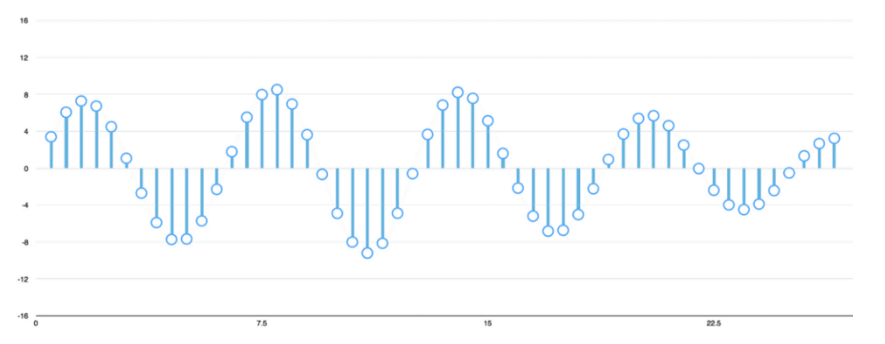
\includegraphics[width=0.9\textwidth]{Figures/onda.png}
	\caption{Onda de sonido \\ Fuente:  \href{https://medium.com/@venkateshpnk22/how-to-convert-your-speech-voice-to-text-data-1b2686099260}{\textit{https://medium.com}}}
	\label{onda}
\end{figure} 
\subsection{Espectro de frecuencias}
Consiste en la distribución de amplitudes para un valor dado de frecuencia de un fenómeno ondulatorio en este caso ondas sonoras.
\begin{figure}[H]
	\centering
	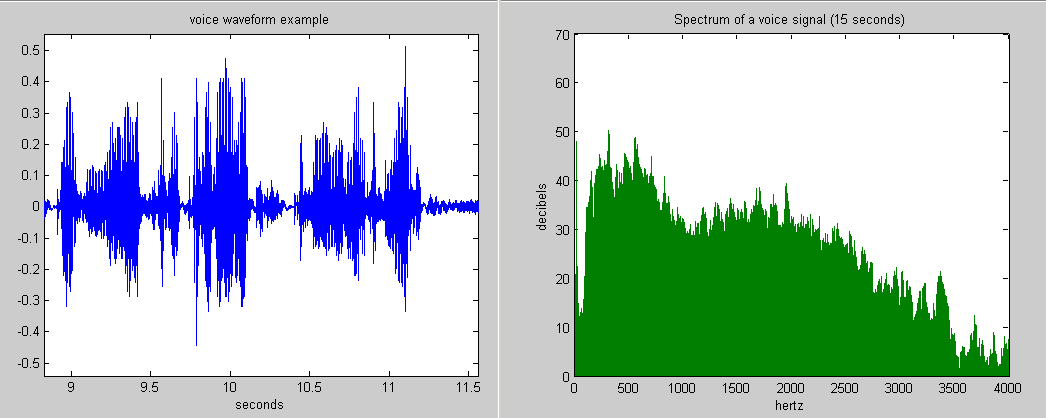
\includegraphics[width=0.8\textwidth]{Figures/espectro.png}
	\caption{señal de voz y su espectro asociado\\ Fuente:  \href{https://www.finaltest.com.mx/product-p/art-03.htm}{\textit{https://www.finaltest.com.mx}}}
	\label{señal}
\end{figure} 

\subsection{Escala mel}
Es una escala psicoacústica propuesta por Stevens, Volkman y Newman. Esta escala es muy importante debido a que la representación más usada en las señales de voz.
\begin{figure}[H]
	\centering
	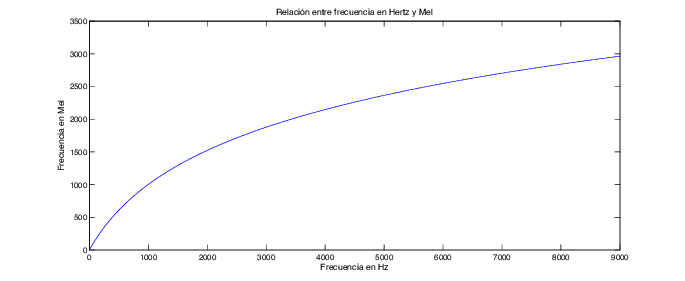
\includegraphics[width=0.8\textwidth]{Figures/escala_mel.png}
	\caption{Relación escala mel - Frecuencia\\ Fuente:  \href{https://www.researchgate.net/figure/Relacion-entre-frecuencia-en-Hz-eje-x-y-en-escala-Mel-eje-y_fig2_312041038}{\textit{https://www.researchgate.net}}}
	\label{mel}
\end{figure} 
\begin{equation}
	\label{STg}
	\begin{aligned}
	m=1127.01048\log_{e}(1+f/700))
	\end{aligned}
\end{equation}
\subsection{Dominio de tiempo}
Este dominio permite obtener la amplitud en un instante de tiempo dado existen dominio de tiempo discretos y continuos.
\subsection{Dominio de frecuencia}
Este dominio permite representar a nuestra frecuencia de onda como un par de amplitud y valores de la fase. Para señales periódicas se relaciona con series de fourier y para señales no periódicas se relaciona con la transformada de fourier.
\begin{figure}[H]
	\centering
	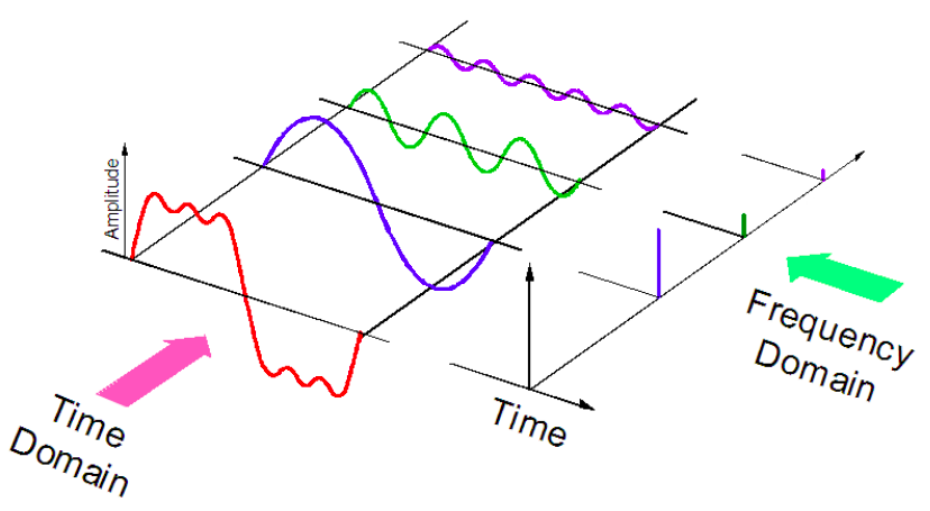
\includegraphics[width=0.6\textwidth]{Figures/audio_signal.png}
	\caption{Dominios de tiempo y frecuencia de dominio\\ Fuente:  \href{https://medium.com/@venkateshpnk22/how-to-convert-your-speech-voice-to-text-data-1b2686099260}{\textit{https://medium.com}}}
	\label{onda}
\end{figure} 


\section{Proceso de extracción de características}

También conocido como análisis de la señal de voz este proceso retené la información necesaria de la voz y elimina los datos redundantes y no necesarios. Este proceso es uno de los más importantes debido a que se transforma la señal en una forma adecuada para los modelos de clasificación. 
\subsection{Etapas del proceso de extracción de carácterísticas}

El proceso de extracción de características puede ser divido en 3 etapas o subprocesos.
\subsubsection{1. Análisis Espectral}
El análisis espectral consiste en descomponer algo complejo en parte o identificar propiedades de la muestra analizada.
Cuando tratamos con una seña de voz esta es variable en el tiempo, por tanto podemos identificar sus características en función a la actividad espectral. El análisis espectral puede ser realizado usando los siguientes métodos:
\begin{itemize}
	\item \textbf{Banco de filtros digitales\\}
	Es un sistema que divide una señal de entrada $x(n)$ en un conjunto de señales $x_{1},x_{2},..$ donde cada una corresponde a una región del espectro de $x(n)$.
	\item \textbf{Transformada de fourier\\}
	Dada una señal aperiódica discreta en el tiempo $x(n)$ definimos la transformada discreta de Fourier como:
	\begin{equation}
	\label{STgl}
	\begin{aligned}
		X(k)=\sum_{n=0}^{N-1}x(n)\exp^{-j2\pi k \frac{n}{N}} k=0, ..., N-1
	\end{aligned}
	\end{equation}
	Esta transformada es calculada por la transformada rápida de Fourier, esta tiene el objetivo de encontrar los componente de la frecuencia en una señal ruidosa dentro de su dominio de frecuencia.
	\item \textbf{Predicción Lineal\\}
	La predicción Lineal o LP, es una técnica para modelar el espectro de la señal de voz por medio de los espectros de todos los polos. \textquotedblleft El método permite la conformación espectral arbitraria en el dominio de la frecuencia y el modelado de espectros continuos y discretos. \textquotedblright \cite{LP}
\end{itemize}


\subsubsection{2. Transformación de parámetros}
Los parámetros son generados mediante operaciones fundamentales como: diferenciación y concatenación. La salida será un vector de parámetros con estimaciones brutas de la señal.
\subsubsection{3. Modelo estadístico }
En este paso se asume que de los parámetros de las señales son producidas por procesos aleatorios multivariados. En este proceso lo único que conocemos es la entrada(parámetros) y la salida. Los vectores de los parámetros son conocidos como observaciones de señales y es usado para determinar si son parte de una palabra, frase o representan un ruido.\\ En la figura 4.5 mostramos el proceso que siguen algunos algoritmos de extracción de características.
\begin{figure}[H]
	\begin{center}
		\begin{tikzpicture}[node distance=2cm]
		\node (i1) [startstop] {Análisis espectral};
		\node (i2) [startstop, below of=i1] {Transformación 	de parámetros};
		
		\node (i3) [startstop, below of=i2] {Modelado estadístico};

		\draw [arrow] (i1) -- (i2) ;
		\draw [arrow] (i2) -- (i3);

		\end{tikzpicture}
	\end{center}
	\caption{Etapas de extracción de características \\ Fuente:  \textit{Fuente Propia}}
\end{figure}
\subsection{Algoritmos}
 A continuación describiremos algunos algoritmos que se usan para realizar este proceso.
\subsubsection{Real Cepstral Coefficient(RCC)}
Este algoritmo convierte la señal del dominio de tiempo a dominio de frecuencia aplicando la transformada rápida de fourier a cada cuadro(frame). Luego se aplica le logaritmo y la transforma de fourier inversa. 
\begin{equation}
\label{STs}
\begin{aligned}
Real Cepstrum = IFFT (log (FFT (s (n))))
\end{aligned}
\end{equation}
Donde:
\begin{itemize}
	\item IFFT: Transformada de fourier inversa
	\item FFT: transformada rápida de fourier.
	\item s(n): señal de voz.
\end{itemize}
\subsubsection{Mel Frequency Cepstral Coefficients (MFCC)} 
Es el algoritmo más usado en aplicaciones de reconocimiento de voz, esta basado en el sistema auditivo humano, el cual es sensible a 2 características dinámicas y estáticas. El MFCC se concentra principalmente en las características estáticas. A continuación describiremos el proceso de la MFCC.
\begin{enumerate}
	\item \textbf{Pre-emphasis\\}
	En este paso la señal pasa a través de un filtro el cual enfatiza las altas frecuencia. Este proceso aumentará la potencia de la señal con mayor frecuencia.
	\item \textbf{Framing\\}
	Se realiza la segmentación de la señal de voz digital, es decir la señal es divida en pequeños intervalos(\textit{frames}), estos generalmente son del rango de 20ms a 30ms.

	\item \textbf{Hamming windowing\\}
	Se utiliza como una forma de ventana que trabajo con los bloques de la cadena de extracción de características y tiene la finalidad de integrar las frecuencias más cercanas.
	\begin{equation}
	\label{STs3}
	\begin{aligned}
	Y(n)&= X(n) x W(n)\\
	W(n)&=0.54-0.46\cos(\frac{2\pi n}{N-1})    0\leq n\leq N
	\end{aligned}
	\end{equation}
	\begin{itemize}
		\item $Y(n)$: Señal de salida
		\item $W(n)$: Hamming window
		\item $X(n)$: Señal de entrada
		\item $N$: Número de ejemplo en cada frame
	\end{itemize}
	\item \textbf{Transformada rápida de Fourier\\} 
	Se encarga de transformar las muestras N del dominio de tiempo al dominio de frecuencia.
	\begin{equation}
		\label{TFF}
		\begin{aligned}
		Y(w)= FFT(H(t)\ast X(t))= H(w) \ast X(w)
		\end{aligned}
	\end{equation}
		\begin{itemize}
			\item $Y(w)$: Transformada de Fourier de Y(t)
			\item $H(w)$: Transformada de Fourier de H(t)
			\item $X(w)$: Transformada de Fourier de X(t)

		\end{itemize}
	
	\item \textbf{Mel filter bank\\}
	Debido a que el rango en el espectro de la Transformada rápida de Fourier es muy amplia y la señal de voz no sigue una escala lineal.
	
	La ecuación 4.5 se usa para calcular Mel para una frecuencia de tiempo.
		\begin{equation}
			\label{TFFs}
			\begin{aligned}
			F(mel)=(2595\ast log10(1+f)700)
			\end{aligned}
		\end{equation}	
		
		
		\begin{figure}[H]
			\centering
			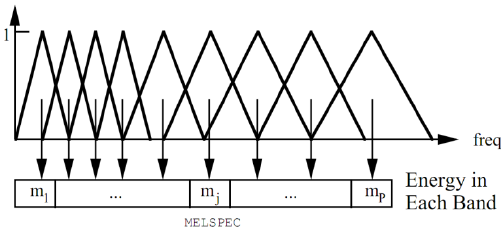
\includegraphics[width=0.7\textwidth]{Figures/melfilter.png}
			\caption{Aplicación del filtro Mel \\ Fuente:  \href{https://www.researchgate.net/figure/Mel-Scale-Filter-Bank-14\_fig2\_280027126}{\textit{https://www.researchgate.net}}}
			\label{onda}
		\end{figure} 
	\item \textbf{Discrete Cosine Transform (DCT)\\}
	Este proceso se encarga de convertir el log del espectro Mel en un dominio de tiempo usando DCT. El resultado es llamado MFCC. El conjunto de coeficientes esa llamado vectores acústicos.
	\item \textbf{Delta energy and Delta spectrum\\}
	La señal de voz junto con los cambios de frames necesitan añadir características relacionadas a los cambios en las características cepstrales sobre el tiempo. La energía en un frame de tiempo $t_{1}$ a $t_{2}$ esta dado por:
	
	\begin{equation}
		\label{energia}
		\begin{aligned}
			Energia=\sum X^{2}(t)
		\end{aligned}
	\end{equation}	
\end{enumerate}
\subsubsection{Codificación lineal predictiva} 
Este método también conocido como LCP considera que la señales de voz pueden ser expresadas como la combinación lineal de las anteriores, entonces podemos describir a la señal de voz utilizando los coeficientes de esta combinación lineal. Este método ha sido utilizado para el procesamiento de la señal de voz debido modela el comportamiento del tracto vocal.\\ En el ecuación 4.3 vemos como se expresa la señal de voz $s$ usando las p anteriores señales de voz y los $a_{k}$ representan \textit{coeficientes del LCP.}

\begin{equation}
\label{LPC}
\begin{aligned}
s(n)= \sum_{k=1}^{p}a_{k}s(n-k)+e(n)
\end{aligned}
\end{equation}



\section{Coincidencia de patrones}
A continuación se describirán algunos algoritmos usados para las tareas de las coincidencias de patrones.

\subsubsection{Modelo oculto de Markov (HMM)}
Es un modelo estadístico donde asumimos que nuestro sistema es un proceso de markov con parámetros desconocidos. A continuación se describirá el proceso en la figura 4.7

\begin{figure}[H]
	\centering
	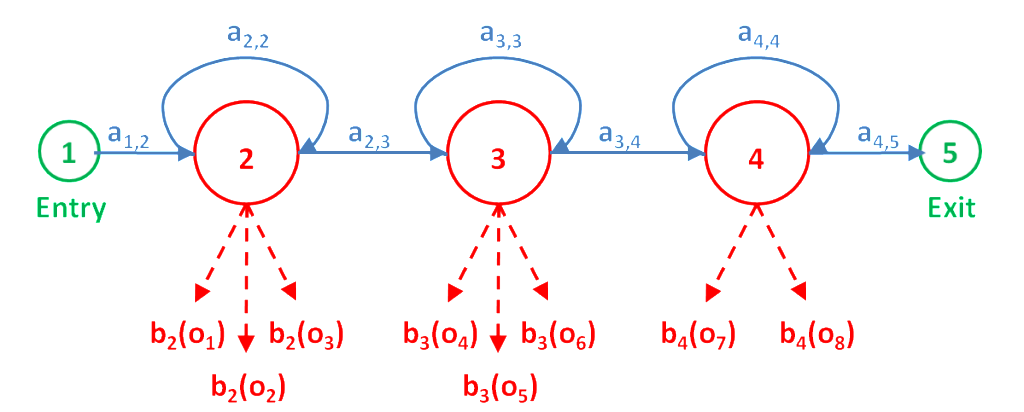
\includegraphics[width=0.6\textwidth]{Figures/hmm}
	\caption{Esquema del HMM\\ Fuente:  \href{http://gekkoquant.com/2014/05/18/hidden-markov-models-model-description-part-1-of-4/}{\textit{http://gekkoquant.com}}}
	\label{}
\end{figure} 
\begin{itemize}
	\item N: Número de estados en el HMM
	\item $a_{ij}$ probabilidad de transición del estado $i$ al $j$.
	\item $	b_{j}(o)$ Probabilidad de generar un vector de característica en estado j.
	
\end{itemize}
\subsubsection{Máquinas de soporte Vectorial(SVM)}
Las SVM usan el concepto de planos de decisión. Un plano de decisión separa un conjunto de objetos que tienes diferentes etiquetas de clases. Las SVM no están restringidas a los problemas lineales debido a las \textit{funciones Kernel.}
\textbf{Funciones Kernels}\\
Las SVM pueden tener distintos tipos de kernels que tienen como objetivo tomar la data y transformarla. Algunas funciones kernels conocidas:
\begin{itemize}
	\item Lineal: $\ker(x_{i},x_{j})= x_{i} \cdot x_{j}$
	\item Polinomial: $\ker(x_{i},x_{j})= ( \gamma x_{i} \cdot x_{j}+C)^d$
	\item Radial: $\ker(x_{i},x_{j})= e^{(\gamma |x_{i} - x_{j}|)}$
	\item Sigmoidal: $\ker(x_{i},x_{j})= \tanh ( \gamma x_{i} \cdot x_{j}+C)$
\end{itemize}
En la figura 4.7 muestra el efecto de las funciones kernels en un conjunto de datos para que este sea linealmente separable sin necesidad de construir curvas complejas.\\
\begin{figure}[H]
	\centering
	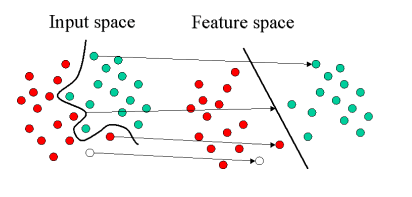
\includegraphics[width=0.9\textwidth]{Figures/svm.png}
	\caption{transformación con la función kernel \\ Fuente:  \href{http://www.statsoft.com/Textbook/Support-Vector-Machines}{\textit{www.statsoft.com}}}
	\label{transformación con la función kernel}
\end{figure} 

\subsubsection{Alineamiento temporal dinámico (DTW)}
Es un método de programación dinámica que busca encontrar una alineación óptima entre 2 series de tiempo. El algoritmo trata de buscar deformaciones entre las series de tiempo y determina la similitudes entre ambas series. Esto nos permite tener una robustez en caso de grupos fonéticos en el audio tenga una duración más prolongada.\\ En la figura 4.6 se muestra 2 series de tiempo donde se trazan las coincidencias entre ambas series.

\begin{figure}[H]
	\centering
	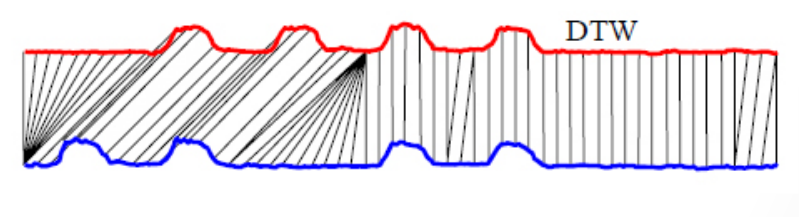
\includegraphics[width=0.9\textwidth]{Figures/dtw.png}
	\caption{DTW\\ Fuente:  \href{https://lemonzi.files.wordpress.com/2013/01/dtw.pdf}{\textit{https://lemonzi.files.wordpress.com}}}
	\label{onda}
\end{figure} 

\subsubsection{Redes Neuronales}
Las redes neuronales descritas en el capítulo 3, luego de su entrenamiento serán capaces de reconocer los patrones de las señales de voz.